\section{The physics of relativistic heavy-ion collisions}

The main objective of relativistic heavy ion physics is to study the nuclear matter under extreme conditions which are high temperature and energy density. In these conditions, the Standard Model anticipates that the nuclear matter undergo a new phase, where the quarks and the gluons are expected to be de-confined called quark-gluon plasma (QGP) and to freely move. %The Standard Model is the theory of the elementary particles and their fundamental interactions. This theory includes the strong interactions due to the color charges of quarks and gluons and a combined theory of weak and electromagnetic interactions.



 %study QCD in a regime of of high temperature, high density, and large reaction volumes. The relativistic heavy ions physics is aimed at the application of this theory to complex and evolving systems of finite size, in order to understand the relations between collective phenomena and the microscopic laws of elementary-particle physics. The collisions between relativistic heavy ions allow to study the nuclear matter under conditions of extremely high temperature and energy density. In these conditions, the Standard Model predicts that the nuclear matter undergo a new phase, where the quarks and the gluons are expected to be de-confined and to freely move. In this context, This phase transition toward this hot and dense state of matter should be accessible to experimental observations. Collisions of atomic nuclei have been studied for more than 20 years at suciently high energies to cross into the deconfined phase. Proposed and developed since the 1960?s, the Standard Model is today a well established theory applicable over a wide range of conditions: the high-energy physics has validated it and confirmed its predictions through a large variety of experiments.The goal is to find conclusive evidence that QCD undergoes a phase transition at a critical temperature from a confined state, where quarks and gluons are bound in colorless hadron states, to a de-confined quark-gluon plasma (QGP), where quarks and gluons can explore volumes larger than the typical hadron radius (R ? 1 fm).



\subsection{Standard model}
If one have question "what the world is made of", our current answer to the question is Standard Model (SM) families \cite{cite:sm} reported in Table \ref{table:particle}. The SM explains the way how those basic blocks of matter interact and how they are ruled by four fundamental forces. In this explanation, the matter consist of 12 particles, which have a spin of 1/2 (fermions) and can be categorized in accordance with way how they interact or equivalently to what charges they carry. The basic particles are six quarks (up, down, charm, strange, top and bottom) that carry fractional charge of $+\frac{2}{3}e$ or $-\frac{1}{3}e$, and six leptons (electron, electron neutrino, muon, muon neutrino, tau, tau neutrino) with integer charge.

\begin{table}[h!]
\centering
\begin{tabular}{llllllll}
\hline
& \multicolumn{3}{c}{Quaks}& \multicolumn{3}{c}{Leptons}\\
Family & Name & Charge[$e$] & Mass & Name & Charge[$e$] & Mass\\
\hline \noalign{\smallskip}
\multirow{2}{4em}1 &   u & 2/3 & 2.2$^{+0.6}_{-0.4}$ \mmass  & $e^{-}$ & $-e$ & 0.511 \mmass\\
&   d & -1/3 & 4.7$^{+0.5}_{-0.4}$ \mmass & $\nu_{e}$ & $0$ & $<$ 2 eV/$c^{2}$\\
\hline \noalign{\smallskip}
\multirow{2}{4em} 2 &   c & 2/3  & 1.27$^{\pm0.03}$\Gmass & $\mu^{-}$ & $-e$ & 105.66 \mmass \\
&   s & -1/3  & 96$^{+8}_{-4}$\mmass & $\nu_{\mu}$ & $-e$ & $<$ 0.19 eV/$c^{2}$\\
\hline \noalign{\smallskip}
\multirow{2}{4em} 3 &   t & 2/3  & 173.21$\pm{1.22}$\Gmass & $\tau^{-}$ & $-e$ & 1.777 \Gmass\\
&   b & -1/3  & 4.18$^{+0.04}_{-0.03}$\Gmass& $\nu_{\tau}$ & $-e$ & $<$ 18.2 \mmass\\
\hline\noalign{\smallskip}
\noalign{\smallskip}
\end{tabular}
\caption{Constituents of matter in the Standard Model}\label{table:particle}
\end{table}

The interactions between elementary particles are described by the exchange of gauge bosons(gluon, photon, Z-boson, W-boson), reported in Table \ref{table:force} together with their relative coupling strengths. The leptons are governed the weak force and the electromagnetic force. Quarks have color property which is the character of charge in the strong force. The color could take one out of three possible values (conventionally red, green and blue). The color can not be appeared freely. After they are confined they come out in the form of hadron which are colorless. Further explaination on color is described in Section \ref{label:qcd}. Then, the hadrons are grouped into baryon and mesons. Baryons consist of three quarks, $qqq$ or ($\bar{q}\bar{q}\bar{q}$) while mesons consist of two quarks ($q\bar{q}$).


\begin{table}[h!]
\centering
\begin{tabular}{lllll}
\hline
Force & Strength & Gauge Boson(s) & Applies on\\
\hline \noalign{\smallskip}
Strong force & 1 &8 Gluons($g$) & Quarks, gluons \\
\hline \noalign{\smallskip}
Electromagetic force &  $\simeq$ 10$^{-2}$ & Photon ($\gamma$) & All charged particles \\
\hline \noalign{\smallskip}
Weak force &  $\simeq$ 10$^{-7}$ & W$^{\pm}$, Z$^{0}$ & Quarks, leptons \\
\hline\noalign{\smallskip}
Gravitation &  $\simeq$ 10$^{-39}$ & Gravitons & All  particles \\
\noalign{\smallskip}
\end{tabular}
\caption{Fundamental forces}\label{table:force}
\end{table}



%\begin{figure}[htbp]
%\begin{center}
%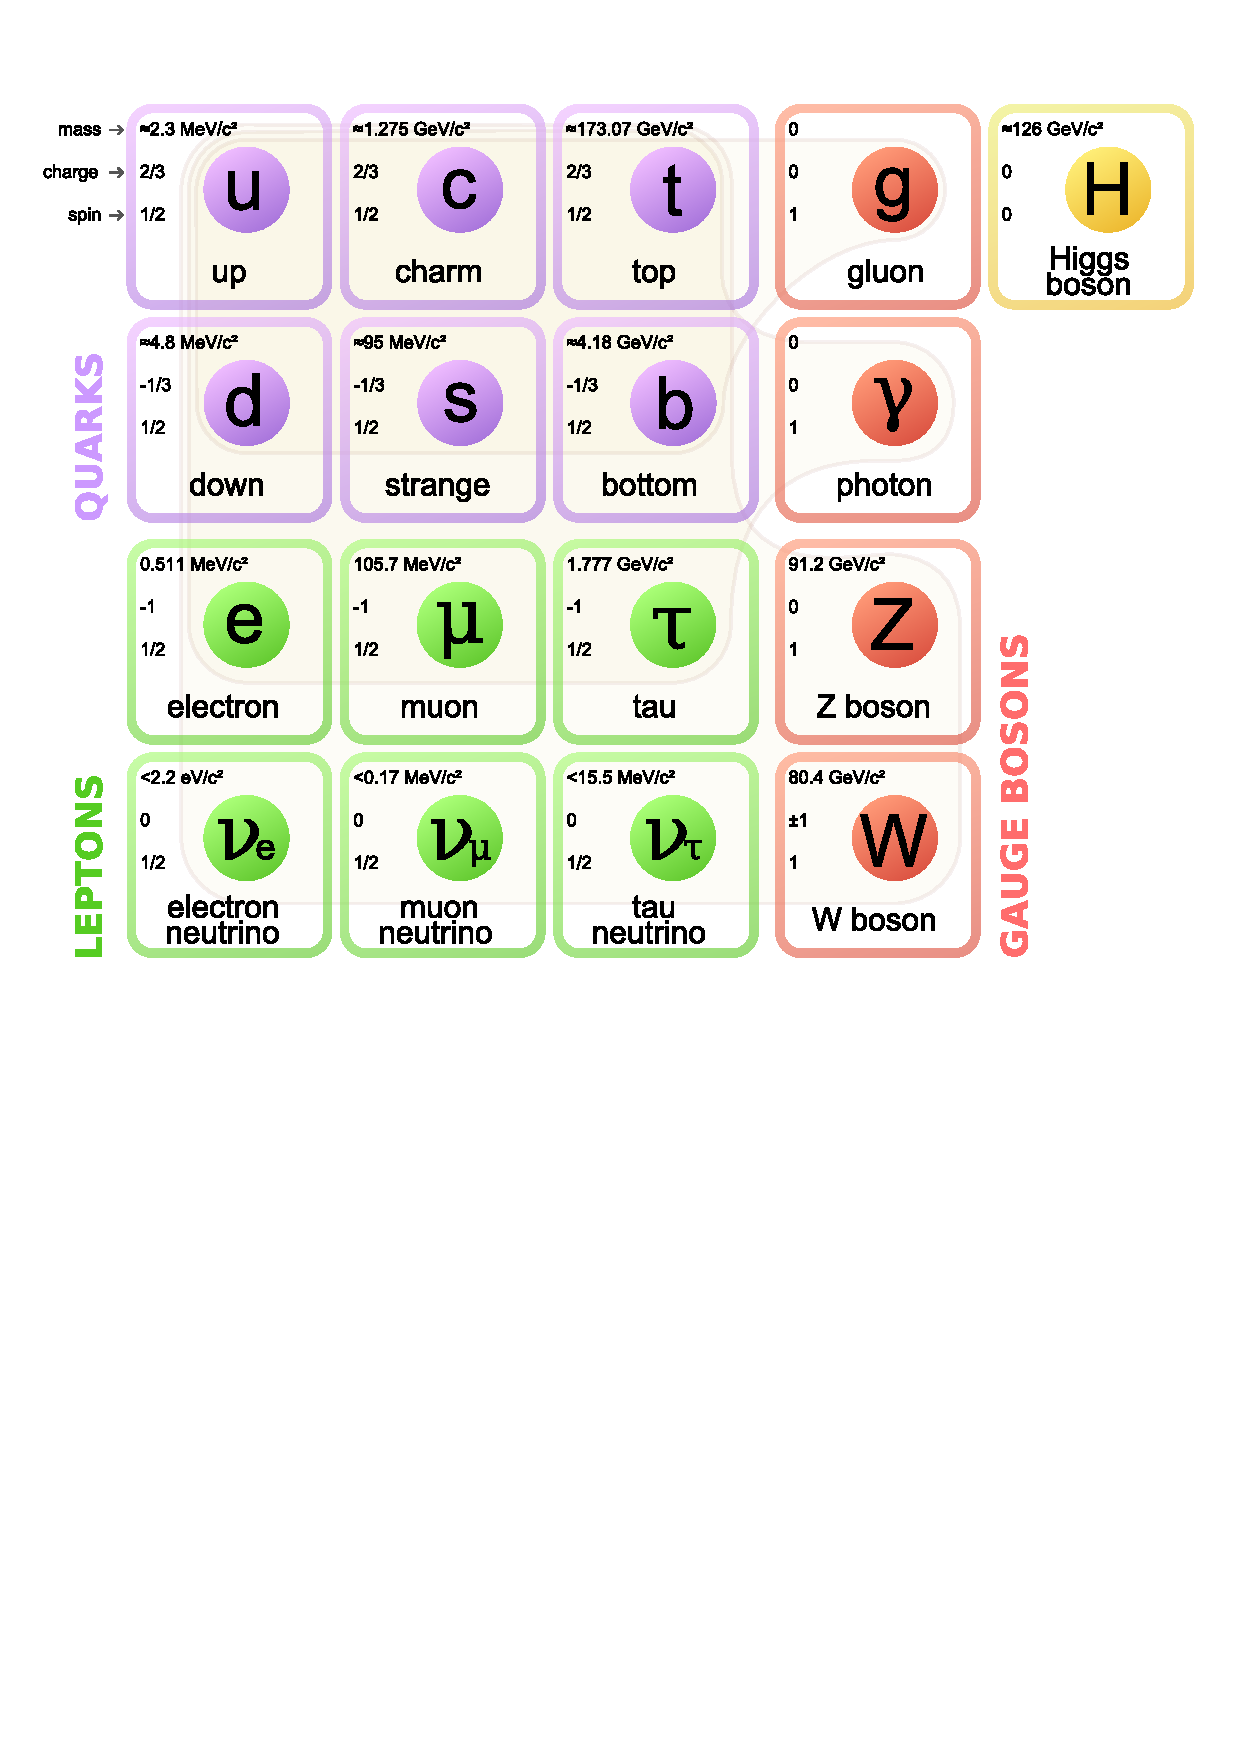
\includegraphics[width=12.cm]{./Version1/FigChapter1/SM}
%\caption{Standard Model families of leptons and quarks as the gauge bosons}
%\label{fig:sm}
%\end{center}
%\end{figure}

%Mathematically, the SM is a quantized Yang-Mills theory based on the non-abelian symmetry group U(1)$\rightarrow$SU(2)$\rightarrow$SU(3) and has a total of twelve gauge bosons: the photon, three weak bosons and eight gluons. The interactions included in such a model are the electromagnetic force, the weak force and the strong one. Quarks have a property called color, playing the role of charge in the strong force. Both quarks and leptons are affected by the weak force and all the charged particles interact electromagnetically.
The models that describe these interactions are listed as follows: \\

\textbf{Quantum Electro-Dynamics (QED)} is a quantum field theory of the electromagnetic force and describes how light and matter interact. This is the first theory where full agreement between quantum mechanics and special relativity is achieved. It explains mathematically not only all interactions of light with matter but also those of charged particles with one another.\\
%It was developed between 1946 and 1950 by Tomonaga Shinichiro, Julian S. Schwinger and Richard P. Feynmann. They were awarded the Nobel prize in 1965. \\

\textbf{Electroweak Theory (EW)} is the unified description of two of the four known fundamental interactions of nature: electromagnetism and the weak interaction. The first measurement of the existence of the weak bosons W$^{+}$, W$^{-}$ and Z$^{0}$ was performed in 1983, when they were produced and directly observed in S$p\bar{p}$S collisions at CERN.\\

\textbf{Quantum Chromo-dynamics (QCD)} is the theory of the strong interaction (color force), describing the interactions between quarks and gluons which make up the hadrons. Starting from the classification of the large amount of particles discovered during the fifties, the original idea of the quark model by Gell-Mann (Nobel Prize in 1969) has been developed during the sixties until 1973, when David J. Gross, H. David Politzer and Frank Wilczek discovered the asymptotic freedom property of the strong nuclear interaction.

\subsection{QCD and Quark-Gloun plasma}\label{label:qcd}
%The strong interaction is one of the four fundamental forces in nature, together with gravity, electromagnetism and the weak interaction. Its existence was postulated in the 1970s, to explain how the atomic nucleus was bound together despite the protons? mutual electromagnetic repulsion. This hypothesized force was called the strong force, which was believed to be a fundamental force that acted on the nucleons. It was later discovered that protons and neutrons were not fundamental particles, by means of deep inelastic experiments, but were made up of constituent particles (the quarks). The strong attraction between nucleons was the side-effect of a more fundamental force that bounds the quarks together in the protons and neutrons. Nowadays the strong inter- action is described through the formalism of a Quantum Field Theory. The particular theory describing this force is the Quantum Chromo-Dynamics (QCD), in analogy to the Quantum Electro-Dynamics (QED) that describes the electromagnetic interaction. In QED the electromagnetic force is mediated by photons, which carry no charge. Similarly, in QCD the gluons are the carriers of the strong force, but unlike the photon they carry color charge, meaning that they can interact with each other. In QED, the electrodynamic coupling constant is $\alpha$ = 1/137, whereas the QCD strong coupling constant, $\alpha_{s}$, can be 1 or larger. In quantum field theory when a coupling constant is much smaller than 1 the theory is said to be weakly coupled. When the coupling nears 1 the theory is strongly coupled, hence the name ?strong? force. In QCD the strong interaction between two quarks can be described using the following potential:
            
As the number of known particle species became large, the idea that these could be the elementary constituents of matter was replaced by the notion that these species could in fact be composite objects made up of fewer, more elementary particles, in a similar way to what had already happened to the elements of Mendeleev's Periodic Table. The original idea by Gell-Mann (1964) was that the hadrons could be obtained as combination of the fundamental representation of an SU$_{f}$(3) group, where three different flavors of quark (q = u, d, s) combine to build mesons ($q\bar{q}$) and hadrons ($qqq$).
However, when cataloging hadrons using the SU$_{f}$(3) group, there are anomalous states, such as the $\Omega^{-}$(sss) and the  $\Delta^{++}$(uuu), that are combinations of three quarks of the same flavor, in clear contrast with the Pauli exclusion principle for fermions. A solution was proposed in 1965 by Moo-Young Han with Yoichiro Nambu and Oscar W. Greenberg, who independently solved the problem by proposing that quarks possess an additional SU(3) gauge quantum number, later called color charge.
This new quantum number may assume three states, represented by the three primary colors: red, green and blue (denoted symbolically by R, G and B, respectively). The introduction of this new quantum number also provides an explanation to other empirical evidence, such as the fact that no $qq$, $\bar{qq}$ or the single quark have never been observed directly. On the other hand, the existence of color charge gives rise to the possible existence of differently colored states for each particle. Thus, we could have many states for the proton, such as u$_{R}$u$_{G}$d$_{B}$, u$_{R}$u$_{G}$d$_{G}$, u$_{B}$u$_{R}$d$_{R}$, and so on. The fundamental rule that solves such contradictions is that all the particle states observed in nature are "colorless" or "white" (or, to be more precise, unchanged under SU$_{c}$(3) rotations).
The dynamics of the quarks and gluons are controlled by the gauge invariant QCD Lagrangian:


\begin{equation}\label{label:L}
\mathcal{L}_{QCD} = \underbrace{i\delta_{ij}\bar{\Psi}^{i}_{q}\gamma^{\mu}\partial_{\mu}\Psi^{j}_{q}}_{\mathcal{L}_{1}}+ \underbrace{g_{s}\bar{\Psi}^{i}_{q}\gamma^{\mu}t_{ij}^{a}A_{\mu}^{a}\Psi^{j}_{q}}_{\mathcal{L}_{2}}+ \underbrace{m_{q}\bar{\Psi}^{i}_{q}\Psi^{j}_{q}}_{\mathcal{L}_{3}}+ \underbrace{\frac{1}{4}F_{\mu\nu}^{a}F^{a \mu\nu}}_{\mathcal{L}_{4}}
\end{equation}

where the coloured gluon field tensor, $F_{\mu\nu}^{a}$ (with color index $a$) and the squared gauge coupling parameter, $g_{s}^{2}$ (associated to the strong coupling constant $\alpha_{s}$) are
defined as:

\begin{equation}\label{label:F}
F_{\mu\nu}^{a} = \partial_{\mu}A_{\nu}^{a} - \partial_{\nu}A_{\mu}^{a} + g_{s}f^{abc}A_{\mu}^{b}A_{\nu}^{c} \end{equation}

and

\begin{equation}\label{label:g}
g_{s}^{2} = 4\pi\alpha_{s}
\end{equation}

where:

\begin{itemize}
\item $\Psi_{q}^{i}$: the quark field with flavor q and color index i $\in$ [1;3], such as $\Psi_{q}$ = ($\Psi_{qR}$, $\Psi_{qG}$, $\Psi_{qB}$)$^{T}$ and $A_{\mu}^{a}$ is the gluon field with color index a (adjoint representation)
\item $\gamma^{\mu}$: Dirac matrices that express the vector nature of the strong interaction, with $\mu$ being the Lorentz vector associated index
\item $m_{q}$: quark mass, a priori not equal to zero (resulting from the Higgs mechanism or equivalent)
\item $t_{ij}^{a}$: generator matrices of the group SU$_{c}$(3), proportional to the Gell-Mann matrices, that perform revolutions in color space, representing interaction of quarks and gluons
\item $f^{abc}$: structure constant of QCD
\end{itemize}

Each of the four terms of the QCD Lagrangian expresses and aspect of the interaction, specifically:

\begin{itemize}
\item $\mathcal{L}_{1}$: gives the kinetic energy of the quark field $\Psi_{q}^{i}$
\item $\mathcal{L}_{2}$: gives the interaction between quarks (fermions) and gluons (the bosons of the interaction)
\item $\mathcal{L}_{3}$: gives the mass of the quarks
\item $\mathcal{L}_{4}$: gives the kinetic energy of the gluons
\end{itemize}

The terms of this equation, together with the fundamental parameters $\alpha_{s}$ and $m_{q}$, summarize in just one expression all the features of the strong interaction. 
The first three terms describe the free propagation of quarks and gluons and the quark-gluon interaction. The remaining two terms show the presence of three and four gluon vertices in QCD and reflect the fact that gluons themselves carry color charge. This is a consequence of the non-abelian4 character of the gauge group.
This peculiarity of the QCD interaction imposes the evolution of the strong coupling constant, $\alpha_{s}$. The corresponding trend has been measured experimentally, and compared in Figure \ref{fig:alpha} with predictions. A practical consequence of this behavior is that the corresponding potential has a completely different shape than the other fundamental interactions and can be expressed by the following equation:


\begin{equation}\label{label:potential}
V(r) = -4\frac{\alpha_{s}}{3r} + kr
\end{equation}

where r is the separation distance between the two quarks and $k$ is a constant that is approximately 1 GeV/fm. %The renormalization scale dependence of the effective QCD coupling $\alpha_{s}$ = $g^{2}_{s}$/4$\pi$ is controlled by the $\beta$-function:

\begin{figure}[htbp]
\begin{center}
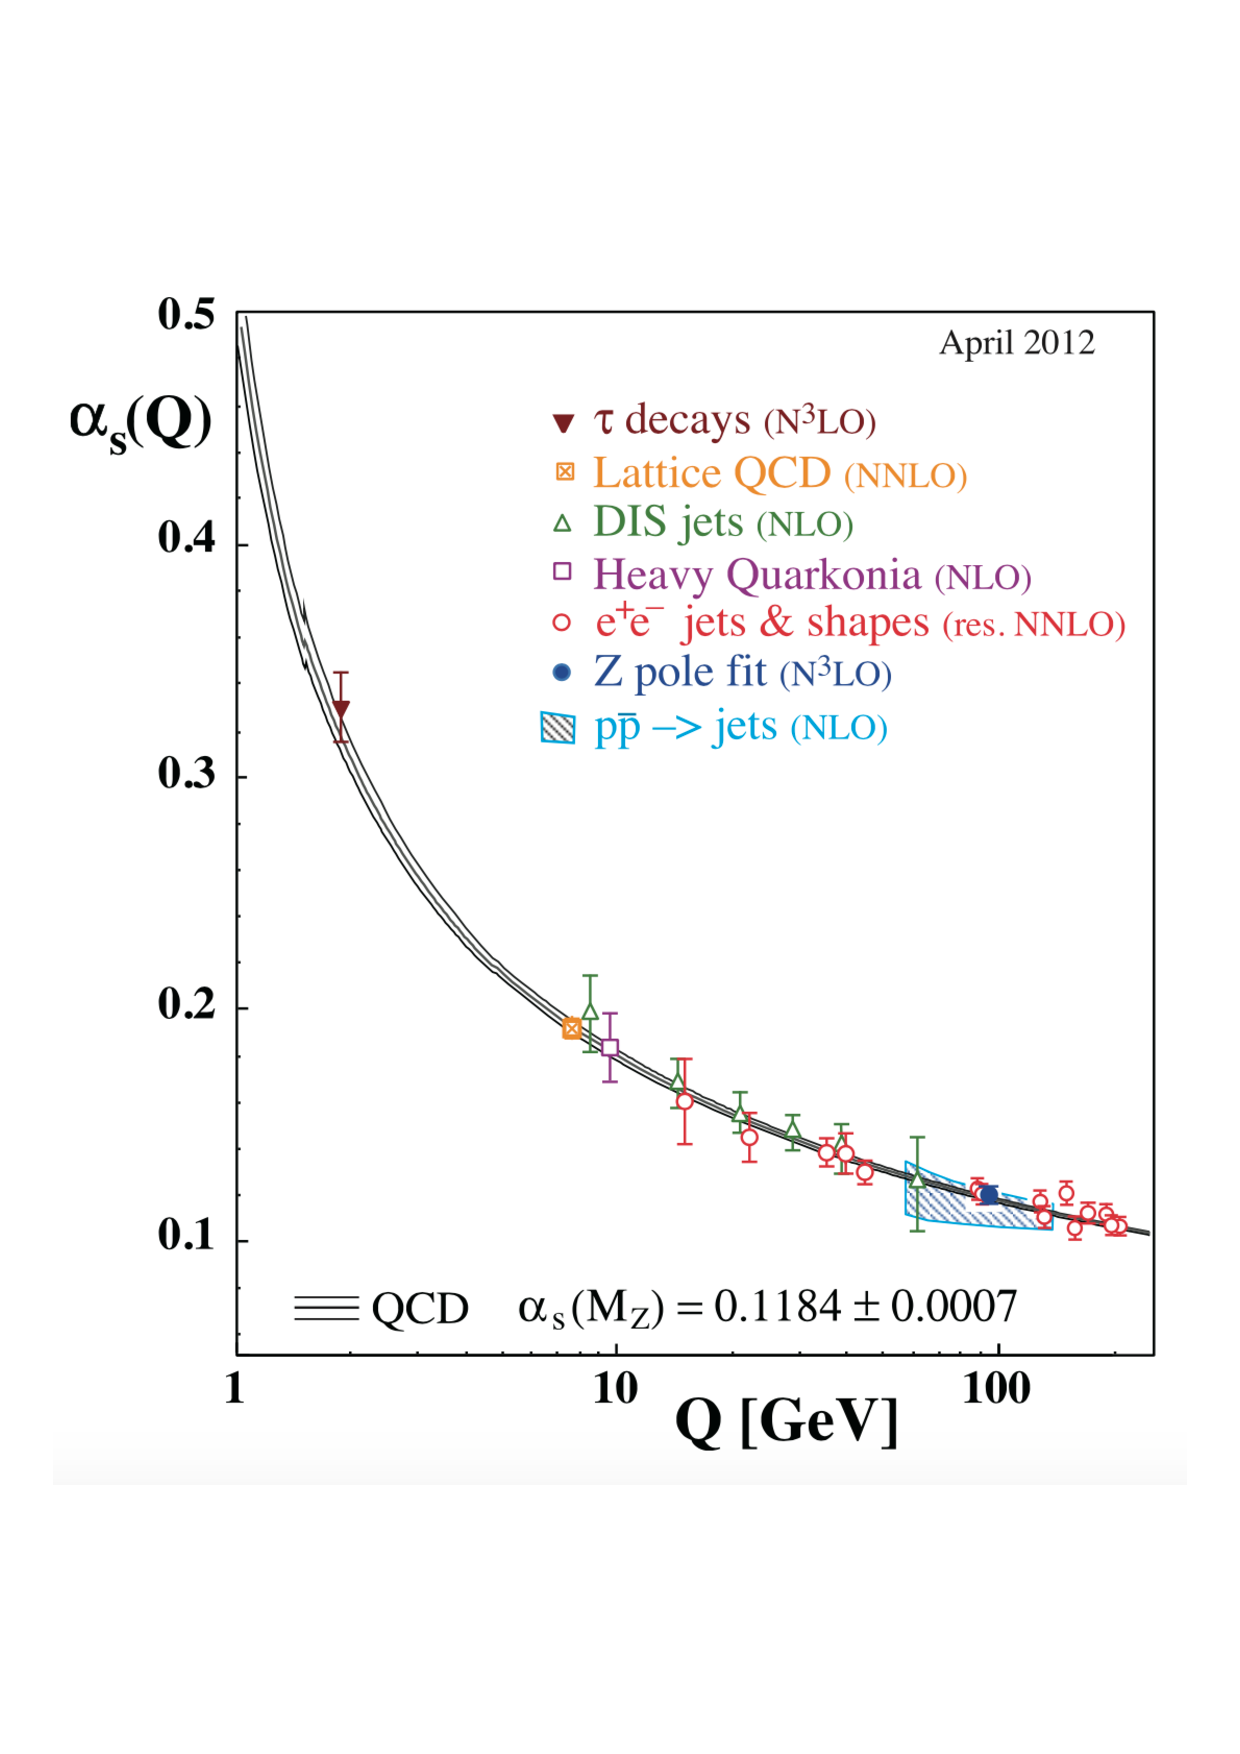
\includegraphics[width=12.cm]{./Version1/FigChapter1/QCD_alpha}
\caption{QCD coupling constant as a function of momentum transfer. Experimental data and also theoretical prediction are presented. \cite{cite:PDG}}
\label{fig:alpha}
\end{center}
\end{figure}

Three are main properties of the QCD interaction: \\

\textbf{Confinement}
At large distances between quarks and gluons (i.e. small values of transferred momentum $Q$ in Figure \ref{fig:alpha}) the coupling constant is large and the associated force is strong enough to keep these elementary con- stituents (usually called partons) confined in bounded states. As expressed in the Equation \ref{label:potential}, the attractive potential increases with the increasing of the relative distance between the two partons preventing the separation of an individual quark or gluon. This explains the meaning of the term "confinement" adopted to describe this energy regime. From the theoretical point of view, the large value of $\alpha_{s}$ make impossible any perturbative approach in the solution of the Hamilton equation of the system. A successful solution is to perform the study of the system on a discrete space. Such techniques are known as lattice QCD and are based on numerical Monte Carlo simulations. The challenge for the calculations is to reduce the lattice spacing in order to approach the continuum.\\

\textbf{Asymptotic freedom}
Reducing the distance between quarks and gluons (i.e. increasing $Q$ in Figure \ref{fig:alpha}) the coupling constant $\alpha_{s}$ becomes smaller. As anticipated, this is a unique feature among the forces and comes from the non-abelian nature of the QCD gauge symmetry. Such a phenomenon is also depicted by the weakening of the anti-screening effect of the surround- ing virtual gluons with decreasing distance. In this way two quarks closer and closer in space show each other a smaller and smaller color charge. \\


\textbf{Chiral symmetry}
One further property of interest is connected to the chirality of the quark. It can be verified that the QCD lagrangian for massless quarks is invariant under a chiral rotation (SU$_{L}$(N$_{f}$) $\times$ SU$_{R}$(N$_{f}$)), while the operator $\bar{q}$q = $\bar{q}_{L}$q$_{R}$ + $\bar{q}_{R}$q$_{L}$ is not invariant (in the axial part), meaning that the mesons (state $\bar{q}$q) should have the same mass. Experimentally this is clearly not true, and it could be shown that the axial current is conserved (PCAC and the Goldberger-Treiman relation). The solution to this puzzle is that the chiral (axial-vector) symmetry is spontaneously broken; this means that the symmetry of the Hamiltonian is not a symmetry of the corresponding ground state. It has also been shown, by G. t?Hooft, that the confinement implies a dynamical breaking of the chiral symmetry. This means that the breaking comes from the interaction between the objects in the system. From this follows that the masses of the quarks are strongly increased because of the interaction with the constituents of the system. This mechanism, known as dynamical chiral symmetry breaking justifies the mass of the hadrons, reducing the role of the Higgs mechanism in the mass explanation at least for the light hadrons.


The asymptotic freedom property suggests the existence of a state of matter, called Quark-Gluon Plasma (QGP), in which the constituents of the hadrons are de-confined. The hatched region in Figure \ref{fig:phase} presents the expected phase boundary between partonic and hadronic matter from lattice QCD calculations. 

Two relevant thermodynamical observables of the system are plotted in the figure. One is temperature T and another one is the baryonic chemical potential $\mu_{B}$. The red points have been measured from thermal models fit on data from different experiment \cite{cite:thermal_pbm} and lie along a line that represent the limit between the two phases. As one can see in Figure \ref{fig:phase}, there are different ways to achieve the transition. It can be performed by changing the temperature and/or the net baryonic density ($\mu_{B}$). 

\begin{figure}[htbp]
\begin{center}
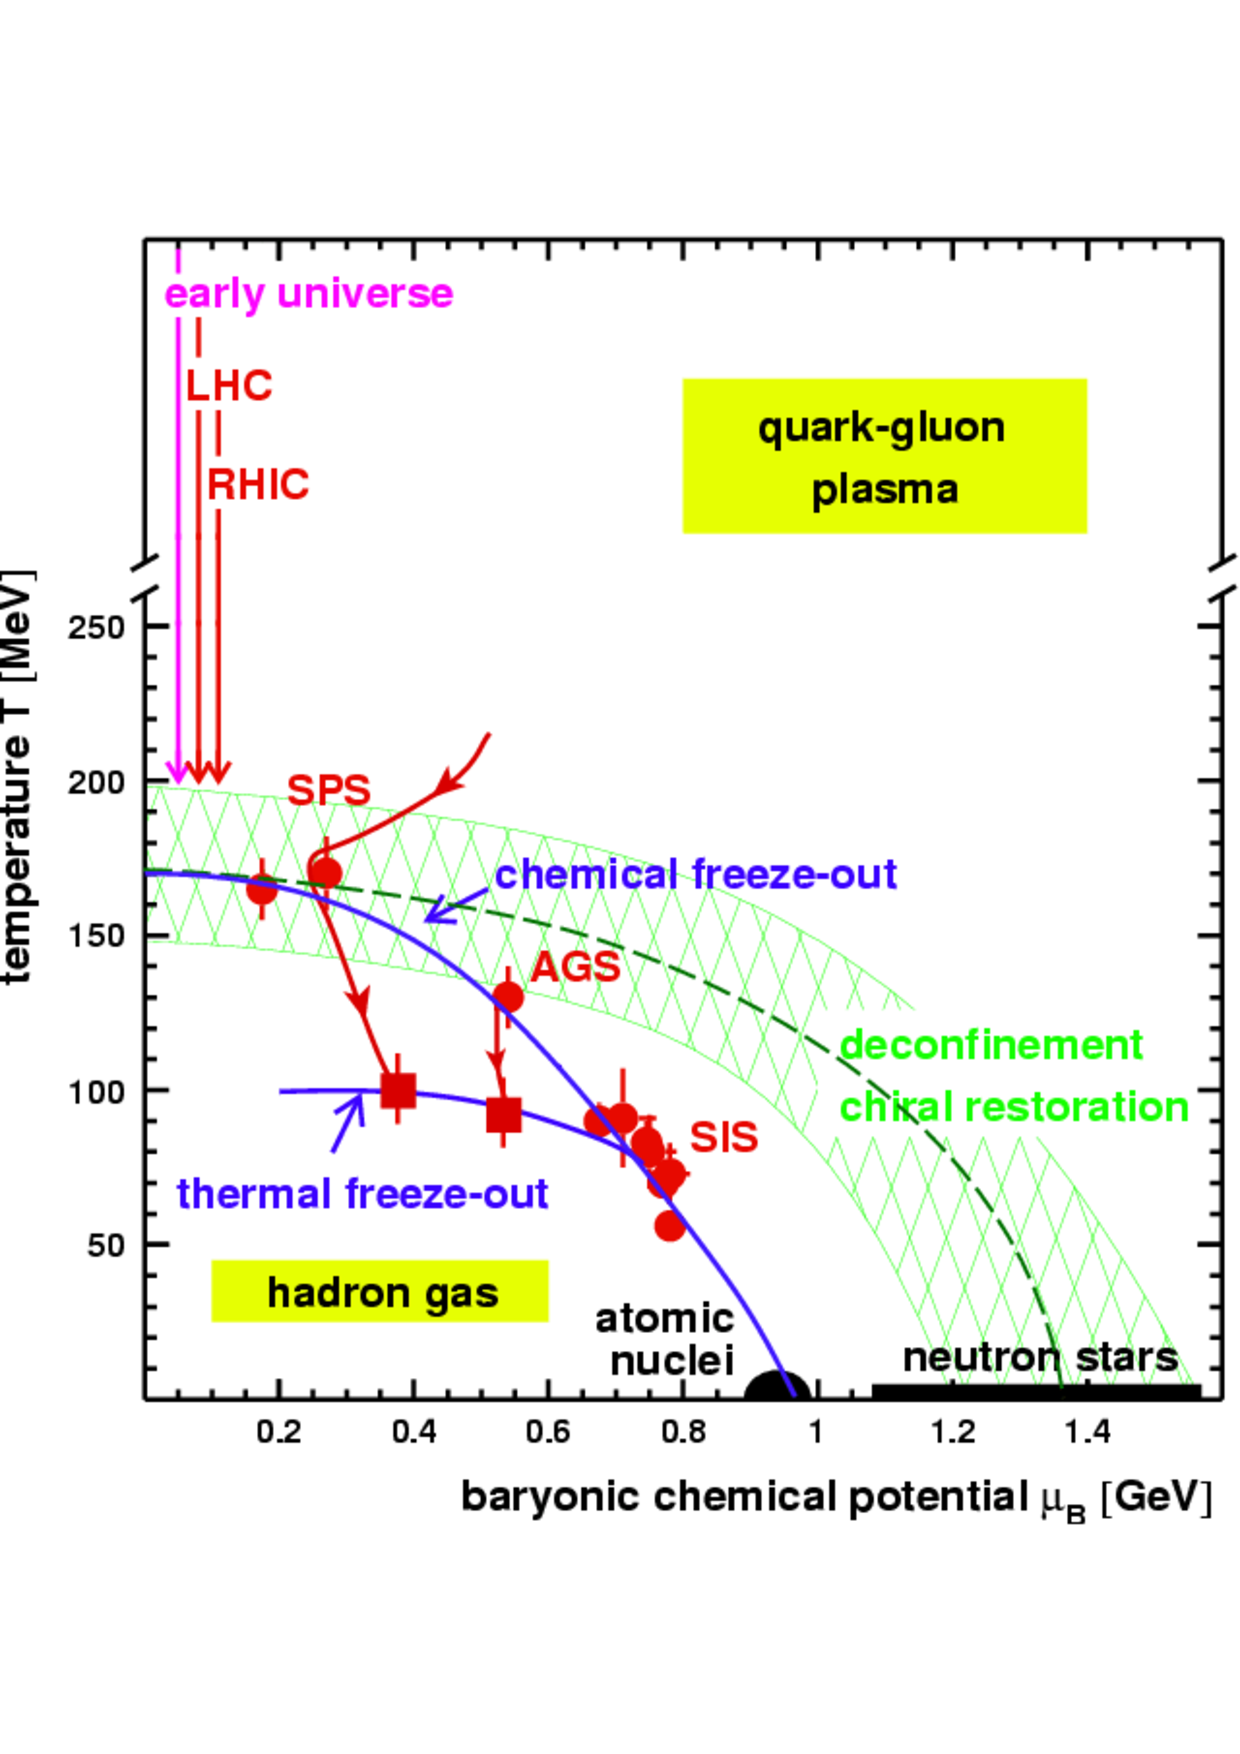
\includegraphics[width=12.cm]{./Version1/FigChapter1/PhaseDiagram}
\caption{Phase diagram of partonic and hadronic matter. The chemical freeze out points are determined from thermal models fit to heavy ion data at SIS, AGS, and SPS energies. (http://na49info.web.cern.ch/na49info/Public/Press/findings.html)}
\label{fig:phase}
\end{center}
\end{figure}


%Experimentally, $\alpha_{s}$ has been measured at different scales ($\mu$). Figure \ref{fig:alpha} shows the measurement of $\alpha_{s}$ as a function of the respective energy scale $Q$ compared to the lattice QCD calculation. Three very important properties of QCD arise from the running constant $\alpha_{s}$. They are confinement, asymptotic freedom, and (hidden) chiral symmetry. For large distance scales the second term in the potential equation (Equation \ref{label:expansions}) dominates. This means that the coupling between the two quarks is large, making it so that no free quarks are observed in nature, i.e. a quark never exists on its own for longer than 1/$\Lambda$QCD, where $\Lambda$QCD = 217 MeV. The up, down, strange, charm, and bottom quarks all hadronize on the time-scale 1/$\Lambda$QCD, the top quark decays before it has time to hadronize. Therefore, all but the top quark will be confined inside hadrons. Experimentally, no single quark in a color- triplet state has ever been observed. Asymptotic freedom arises when the quarks are at a small distance from one another or with a large enough momentum transfer $Q$ ($\alpha_{s}$ $\rightarrow$ 0 as $\mu$ $\rightarrow$ $\infty$). The potential will go like 1/r and the effective coupling between the quarks decreases, allowing for a quasi-free quark. The third property is called chiral symmetry, also not observed in nature. It is a symmetry of QCD in the limit of vanishing quark masses. In this limit quarks are either left of right handed, such that the QCD Lagrangian is symmetric. However, when quarks are confined inside hadrons they have large dynamical masses, called constituent or QCD masses. Here the chiral symmetry is said to be ?broken? (or hidden). In the small ?s limit some quarks will have small mass, called current mass. In this limit, chiral symmetry is said to be (partially) restored. In our world, quarks and gluons are confined inside hadrons. By significantly increasing the temperature and energy density the strong force holding the quarks and gluons together may be reduced, unbinding them from the hadrons. This phenomenon is known as "de-confinement". De-confinement implies that there exists a phase transition from a gas of hadrons to a new form of matter of free quarks and gluons, called the Quark-Gluon Plasma (QGP).

\newpage
\subsection{Heavy Ion Collisions}

Knowledge of the space-time evolution of the system created in high energy heavy ion collisions help to understand the dynamics of nuclear matter under extreme conditions. 
The Figure \ref{fig:HI} presents the schematic of the time evolution in case of collision of two Lorentz contracted nuclei at very high energy. After the colliding, a large amount of energy can be deposited in a small area of space and in a short duration of time. The matter produced might have very high energy density and temperature so that it is sufficiently able to reach to QGP that is baryon free region.

Just after the colliding, the medium may not be in thermal equilibrium which can be reached after that the evolution is governed by the low of thermodynamics. As the system expands and cools, the hadronization takes place and and the freeze out comes after some time.
Different stages during the collisions can be studied by various observables, such as, Electromagnetic probes,  Quarkonia and heavy flavour, Hard probes, Electroweak probes, global properties and Freeze-out condition as well. Most of the produced particles in the high energy heavy-ion collisions are emitted at freeze-out. In order to estimate the energy density, pressure, temperature and baryon chemical potential, the study of particle after freeze-out gives crucial information. Those quantities could be derived from measurement of multiplicity and rapidity distribution, transverse momentum (\pt) distributions.


\begin{figure}[htbp]
\begin{center}
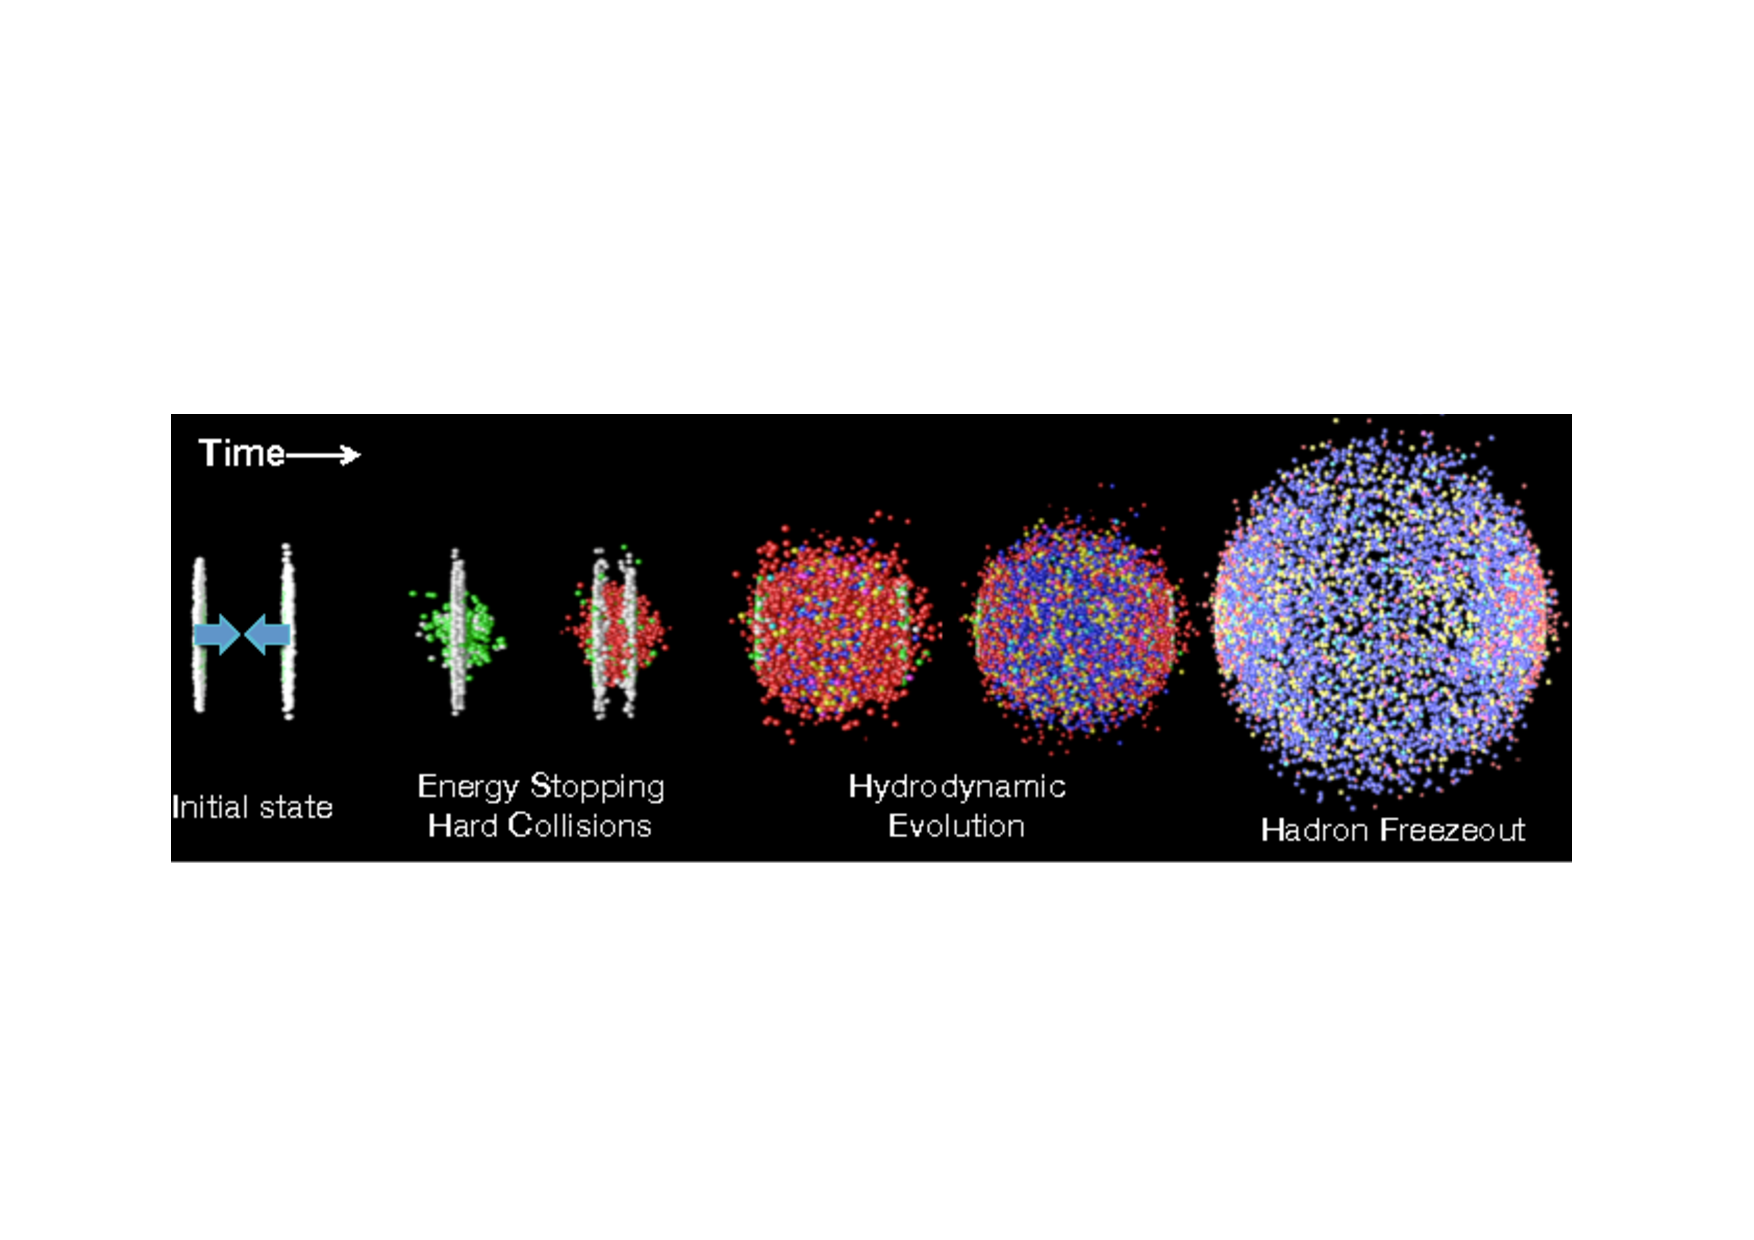
\includegraphics[width=12.cm]{./Version1/FigChapter1/HI}
\caption{The time evolution of a high energy heavy ion collision. \cite{cite:HI}}
\label{fig:HI}
\end{center}
\end{figure}

In the case a QGP is formed, it will eventually expand because of its internal pressure. As the system expands it also cools. The space-time evolution of the expansion can be seen in Figure \ref{fig:freezeout} (right side). A and B represent the two incoming ion beams. After a pre- equilibrium phase a QGP is formed. As it expands, the system will eventually reach what is known as the critical temperature ($T_{c}$). At this point partons begin to hadronize and this will continue until the chemical freeze-out ($T_{ch}$) takes place, when inelastic collisions cease. At this stage the distribution of hadrons is frozen. As cooling and expansion continue the hadrons reach what is called thermal freeze out ($T_{fo}$). Here the elastic collisions stop and the hadrons carry fixed momenta. The QGP state can not be directly observed, because of its short lifetime. Instead, through experiment we measure the final state hadrons, which have a fixed momentum after $T_{fo}$. The observables of interest should tell us about the de-confinement and the thermodynamic properties of the matter. Moreover, experimental measurements include yields and \pt spectra of various particle species, azimuthal studies of high \pt particles, phase space distributions, and particle correlations.

\begin{figure}[htbp]
\begin{center}
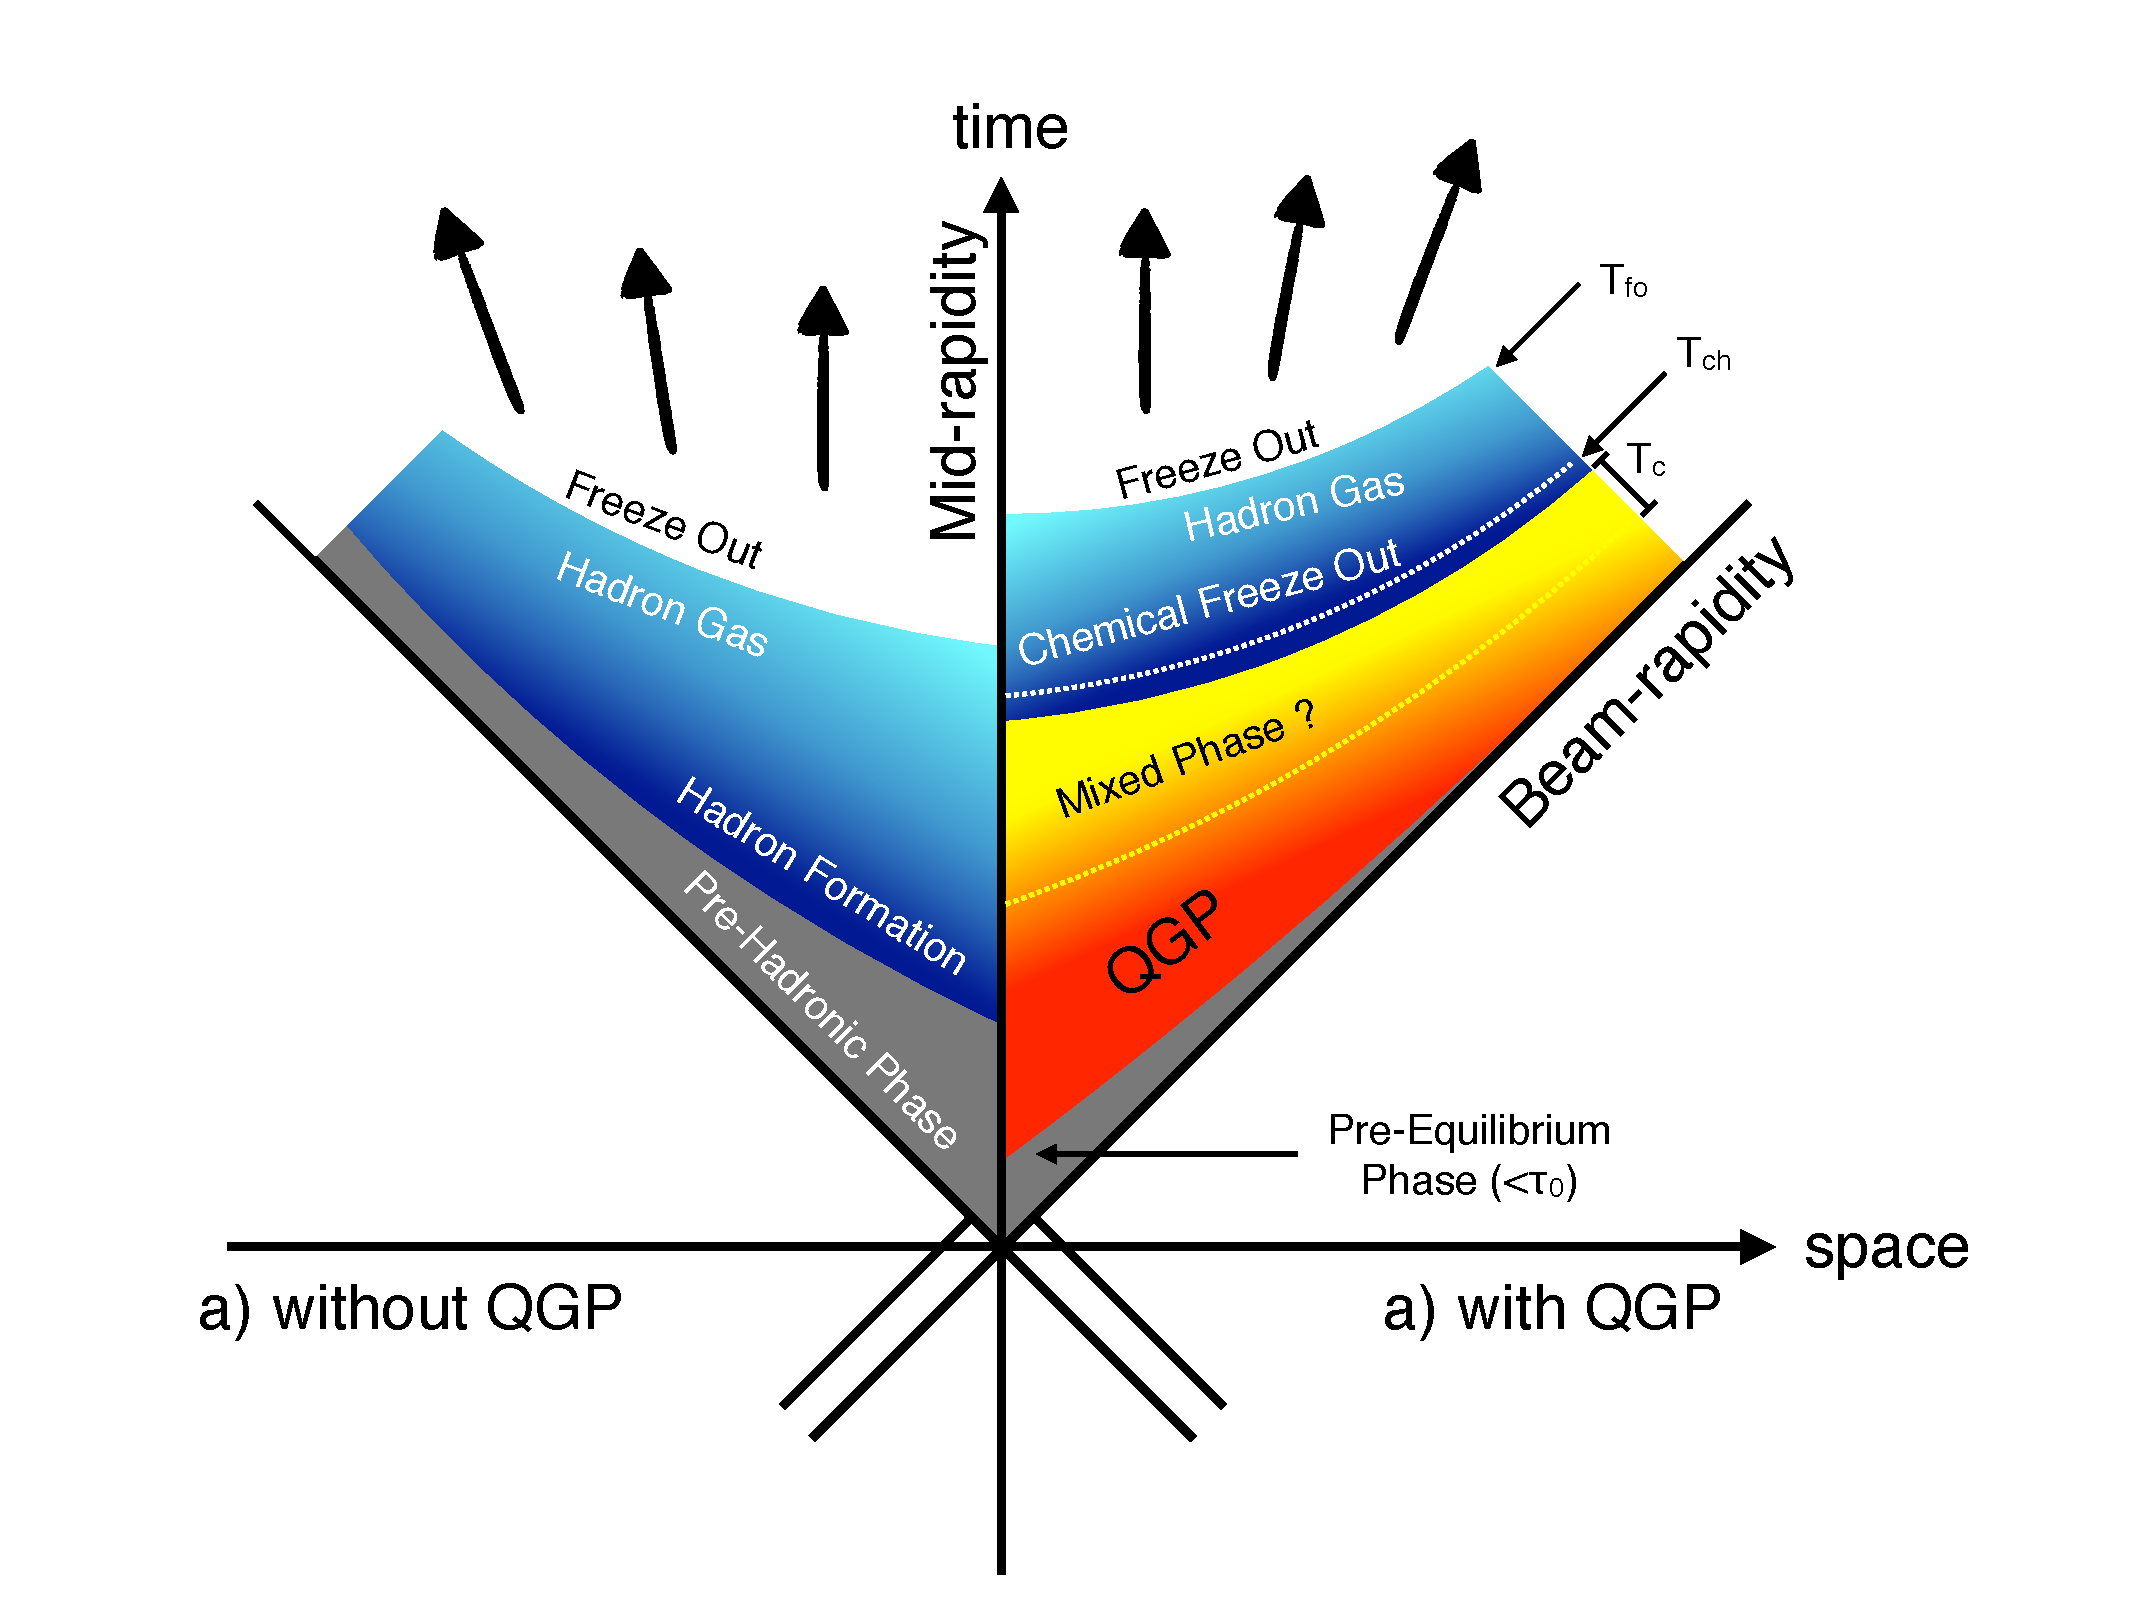
\includegraphics[width=18.cm]{./Version1/FigChapter1/FreezeOut}
\caption{Hydrodynamic evolution of a heavy ion collision with and without the formation of a QGP. }
\label{fig:freezeout}
\end{center}
\end{figure}

A practical way to reach a critical condition in which a nuclear system should undergo a phase transition to the QGP, at high temperature and/or matter density, is to collide two nuclei at sufficiently high energy. Therefore, relativistic and ultra-relativistic heavy-ion collisions are a unique tool to study nuclear matter under extreme conditions.



%Three snapshots illustrating a nuclear collision of two nuclei. (Left frame) The two incident nuclei are Lorentz contracted as the incident velocities are already close to the speed of light. (Middle frame) The moment of highest compression. (Right frame) The expansion stage, when most of the particles already no longer interact strongly.


\newpage